\documentclass[12pt, a4paper, oneside]{ctexart}
\usepackage{amsmath, amsthm, amssymb, graphicx}
\usepackage[bookmarks=true, colorlinks, citecolor=blue, linkcolor=black]{hyperref}
\usepackage[margin = 25mm]{geometry}
\usepackage{setspace}
\usepackage{graphicx}

% 导言区
\title{The renaissance of jet physics report}
\date{\today}
\author{202011010101 物理2001 孙陶庵}
\begin{document}
\begin{spacing}{2.0}
\maketitle
\section{introduction}
本文主要研究Zhongbo Kang老师于2022/06/20在湖南大学的演讲内容,即有关射流(jet)的研究。
在高能粒子对撞机中,两个(或多个)粒子碰撞后会朝着某一特定方向前进,而其反射出来的粒子一般为胶子或夸克。
射流是在 量子色动力学(QCD) 散射过程中产生的,产生高横向动量夸克或胶子。产生特定射流的概率由射流产生截面描述,
它是基本微扰 QCD 夸克、反夸克和胶子过程的平均值,由部分子分布函数加权。
对于最频繁的射流对产生过程,即两个粒子的散射,强子碰撞中的射流产生截面由下式给出
\begin{center}
  $\sigma_{i j \rightarrow k}=\sum_{i, j} \int d x_{1} d x_{2} d \hat{t} f_{i}^{1}\left(x_{1}, Q^{2}\right) f_{j}^{2}\left(x_{2}, Q^{2}\right) \frac{d \hat{\sigma}_{i j \rightarrow k}}{d \hat{t}}$\\  
\end{center}
$x, Q^2$:纵向动量分量和动量传递\\
$\hat{\sigma}_{i j \rightarrow k}$:反应 ij → k 的微扰 QCD 截面\\
$f_{i}^{a}\left(x_{a}, Q^{2}\right)$:用于在光束 a 中找到粒子种类 i 的部分子分布函数。 \\
微扰 QCD 计算可能在最终状态下具有有色部分,但只有最终产生的无色强子是通过实验观察到的。
因此,为了描述作为给定过程的结果在探测器中观察到的内容,所有输出的有色部分必须首先经历部分子簇射,
然后将产生的部分组合成强子。术语碎片化和强子化在文献中经常互换使用,以描述软 QCD 辐射、强子的形成,
或同时使用这两种过程。
在相对论重离子物理学中,射流很重要,因为原始硬散射是碰撞中产生的 QCD 物质的自然探针,
并指示其相位。当 QCD 物质经历相交叉进入夸克胶子等离子体时,介质中的能量损失显着增加,有效地降低了射流的强度。

射流分析技术的例子有:

射流相关
风味标记(例如,b 标记)
射流子结构。
由於量子色動力學 (QCD) 限制只允許無色狀態,因此攜帶顏色電荷的粒子(例如夸克)不能以自由形式存在。
當一個含有色荷的物體發生碎片時,每個碎片都會帶走一些色荷。為了服從限制,這些碎片在它們周圍創造出其他有色物體,
形成無色物體。這些物體的集合稱為射流,因為碎片都傾向於沿同一方向行進,形成狹窄的粒子“射流”。射流在粒子探測器中被測量和研究,
以確定原始夸克的性質。

\section{Begining of jet physics}
对于射流的研究是非常早的,George Strman 于1977发布的"Jets from Quantum Chromodynamics"\cite{PhysRevLett.39.1436},
其主要为$e^+$和$e^-$ 的碰撞反射出两个方向(back to back)的夸克()。 \\
而同样在大约1979,"Search for gluons in $e^+e^-$ annihilation"\cite{ELLIS1976253} 用了类似的作法找到了胶子,
当能量足够大时,末态出来的夸克有可能分离出胶子。

\begin{figure}[htbp]
	\centering
	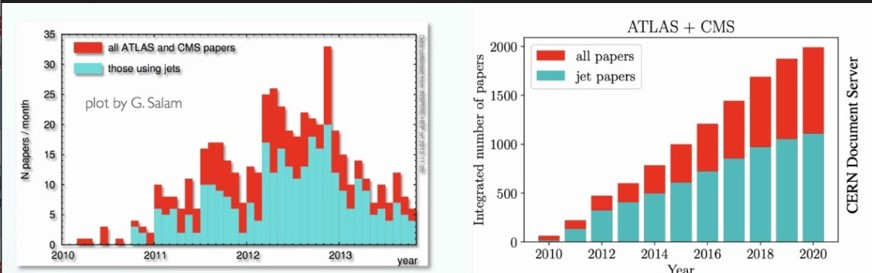
\includegraphics[width=8cm]{sigma.jpg}
	\caption{statistics graph 1 by report}
\end{figure}
\subsection{What are we using jets for?}
\subsubsection{Quantum imaging of protons and nuclei}
就像黑洞成像显示引力动力学一样,质子成像将提供对强相互作用的见解,特别是在与质子大小相对应的动量尺度上,
再藉由3D成像分析粒子自旋,或许也可以在MRI上有所作用。
亚原子粒子具有自旋的量子力学性质。某些原子核,如 1H(质子)、2H、3He、23Na 或 31P,具有非零自旋,因此具有磁矩。
对于所谓的自旋 1⁄2 原子核,例如 1H,有两种自旋状态,有时称为向上和向下。

当这些自旋被置于强大的外部磁场中时,它们会沿着磁场方向围绕轴进动。质子以两种能量本征态排列(塞曼效应):
一种低能和一种高能,它们被非常小的分裂能分开。
MRI 主要用于诊断医学和生物医学研究,但它也可用于形成无生命物体的图像,例如木乃伊。除了详细的空间图像外,
扩散 MRI 和功能 MRI 扩展了 MRI 的实用性,
当在磁铁内部时,质子倾向于对齐,并且它们也围绕自己的轴旋转,因为与电荷结合的自旋在经典上被视为具有自己的磁偶极矩,
就像一个小条形磁铁.就像引力场中的陀螺仪一样,有一个快速旋转。然而,在重力施加的扭矩下,陀螺仪会围绕主重力场方向摆动或“进动”。
这种经典解释在单个核自旋尺度上被认为是不现实的;然而,结合足够多的原子核,进动磁化矢量的经典模型已被证明是有效的,并且被称为群体行为模型,用以
以分别捕获神经系统中的神经元束和血流。极大地推动了医学、神经生理学和认知神经科学的迅速发展。
\subsubsection{A New Glassy State of Matter: The Color Glass Condensate}
首先,色荷是夸克和胶子的一种性质,与量子色动力学(QCD)理论中粒子的强相互作用有关。
夸克和胶子的“颜色电荷”与颜色和电荷的日常含义完全无关。术语颜色和红色、绿色和蓝色标签变得流行,仅仅是因为与原色的松散类比。
有些粒子有相应的反粒子。具有红色、绿色或蓝色电荷的粒子具有相应的反粒子,其中色电荷必须分别是红色、绿色和蓝色的反色,
以便在粒子-反粒子的产生和湮灭中保持色电荷。粒子物理学家称这些为反红、反绿和反蓝。所有三种颜色混合在一起,
或这些颜色中的任何一种及其补色(或负),是“无色”或“白色”,净色荷为零。由于称为颜色限制的强相互作用的特性,
自由粒子的颜色电荷必须为零:重子由三个夸克组成,它们必须是红色、绿色和蓝色中的一种;
同样,一个反重子由三个反夸克组成,反红、反绿和反蓝各一个。介子由一个夸克和一个反夸克组成;
夸克可以是任何颜色,反夸克有相应的反色。
而jet physics可以帮助观察到固体、液体、气体、等离子体和玻色-爱因斯坦凝聚态以外的第六态有色玻璃凝聚物。 \cite{https://doi.org/10.1111/ijag.12013}
\subsubsection{jet propagation in nuclear matter}
在重离子反应中,射流被广泛用作探针在夸克-胶子-等离子体(QGP)的研究。
射流在介质中的传播也会影响强相互作用核物质性质的测量。
进而影响高能夸克和胶子致密 QCD 物质中的传播和相互作用。 \cite{Ovanesyan_2011}
包含射流横截面和射流电荷的理论研究
电子离子对撞机。预测电子金中这些可观测物相对于
电子 - 质子碰撞揭示了灵活的质心能量和运动覆盖率如何
未来电子离子对撞机中与原子核反应的射流产生和射流子结构将发挥重要作用
在核结构探索和部分子阵雨演化中的杰出作用
相互作用的物质。 在软共线有效理论的框架下,推广到包括in-medium
相互作用,
同时也可以从理论上证明了如何解开核子分布的影响功能以及由jet和核之间的最终状态相互作用产生的功能\cite{PhysRevLett.126.252001}
\begin{figure}
    \begin{minipage}[t]{0.5\linewidth}
        \centering
        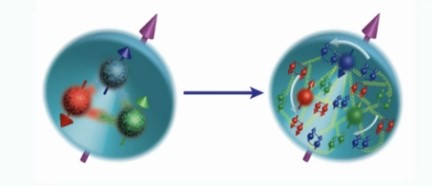
\includegraphics[scale=0.3]{kappa.jpg}
        \caption{Quantum imaging of protons and nuclei}
        \label{fig:side:a}
      \end{minipage}%
      \begin{minipage}[t]{0.5\linewidth}
        \centering
        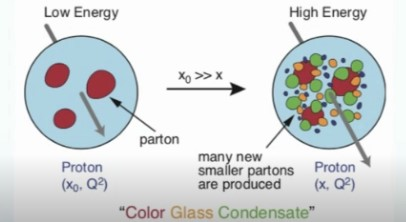
\includegraphics[scale=0.3]{mu.jpg}
        \caption{A new form of matter - color glass condensate}
        \label{fig:side:b}
      \end{minipage}
\end{figure}
\begin{figure}
    \centering
    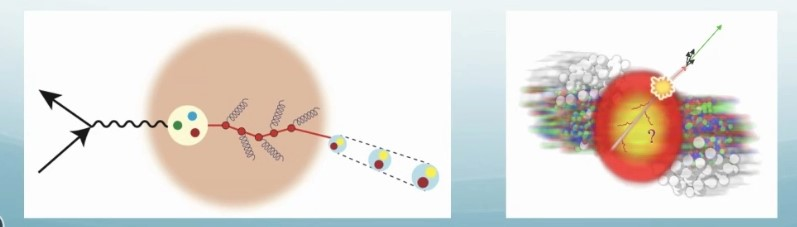
\includegraphics[width=8cm]{nu.jpg}
    \caption{jet propagation in muclear matter}
\end{figure}

\subsection{imaging a proton}
研究黑洞的过程我们发现了引力波,而研究质子可以让我们发现强力(strong interaction)的内在作用,
我们现在的问题是\\
(1)如何从基本夸克/胶子中产生核子的性质,例如质量和自旋\\
(2)夸克自旋与质子自旋之间的量子相关性
\subsubsection{fundamental structure of proton?}
虽然质子最初被认为是基本粒子,但在现代粒子物理学标准模型中,质子现在被称为复合粒子,包含三个价夸克,现在与中子一起被归类为强子。
根据标准模型,质子由三个夸克组成:两个上夸克和一个下夸克。这些夸克结合起来赋予它电荷和自旋。
质子的 +1 电荷来自两个上夸克(每个 $+\frac{2}{3}$)和一个下夸克($-\frac{1}{3}$)的组合电荷。三个夸克被强大的力量结合在一起; 
这些键的能量决定了质子的大部分质量。因为质子由三个结合在一起的夸克组成,所以它是重子。中子也是重子,由两个下夸克和一个上夸克组成
,因此没有净电荷。

\section{Connecting theory and experiment}
这一部分在理论范围内使用了现象学(Phenomenology/唯像学)的工作,从实验数据中得到质子在夸克方面的联系,对图(a)可以设计实验

\begin{figure}
    \centering
    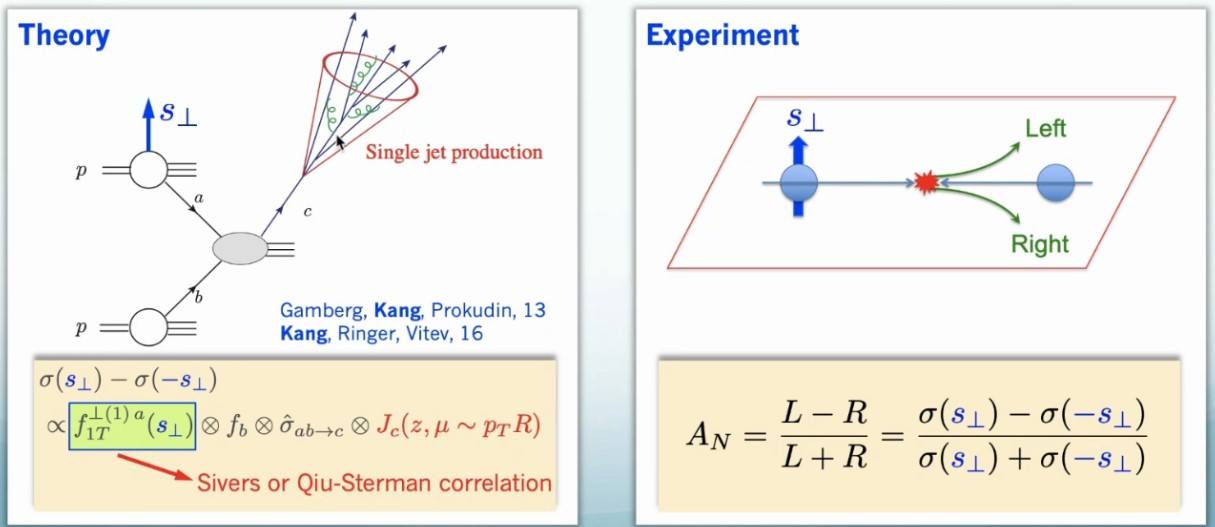
\includegraphics[width=8cm]{theory and experiment.jpg}
    \caption{the comparation of theory and experiment}
\end{figure}


%这里非常重要一定要展开!!!!!
\subsection{Experiment introduce}
可以将两个质子相互作用他们的末态会产生一个射流,此时我们可以尝试对一个质子探测我们需要的关联,对各个粒子进行观测建构出几个关系式,
这一部分在理论范围内使用了现象学的工作,这样我们就只需要和实验数据比对就行。
但是我们可以发现对于single jet而言,他的动量大约在60GeV-100GeV之间,而我们关联的横向动量约在1GeV,这样我们就会观察不到,
对此,可以改进实验方法,
在实验中进一步测量小的横向动量,例如 dijet 中的横向动量($q_T$)的不平衡(见图b)从而建构一个有效的场理论
\begin{figure}
    \centering
    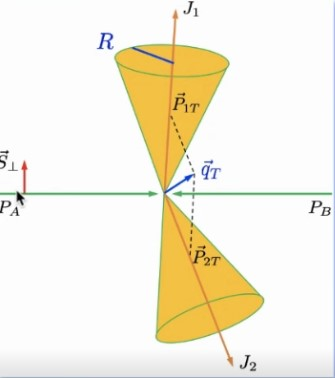
\includegraphics[width=8cm]{delta.jpg}
    \caption{Improvements to experiments}    
\end{figure}

\subsection{Experiment data}
我们从实验数据可以看出,无论是singlejet 或dijet的数据都是十分接近0的。
这说明在刚刚的实验前提下得到的结果会有一种相互抵消的状况出现
\begin{figure}
    \begin{minipage}[t]{0.5\linewidth}
        \centering
        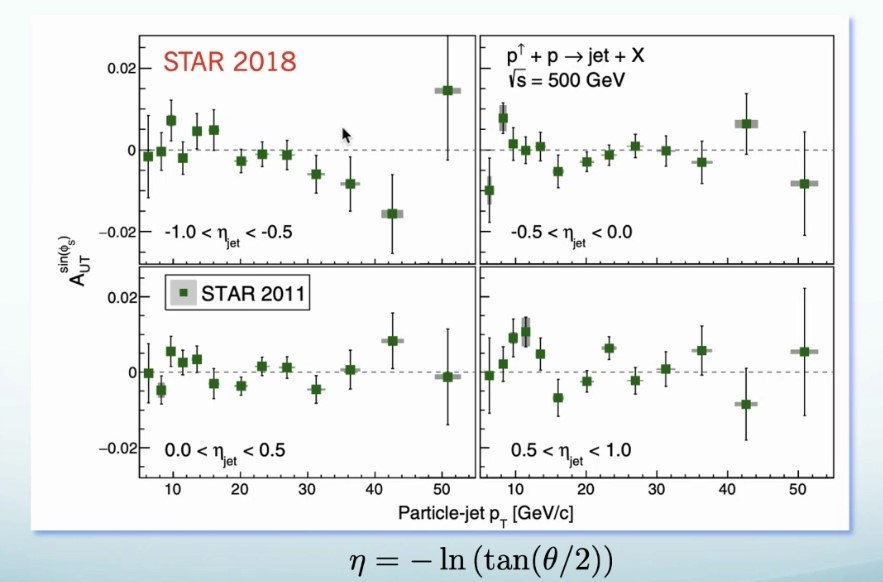
\includegraphics[scale=0.3]{alpha.jpg}
        \caption{singlejet}
        \label{fig:side:a}
      \end{minipage}%
      \begin{minipage}[t]{0.5\linewidth}
        \centering
        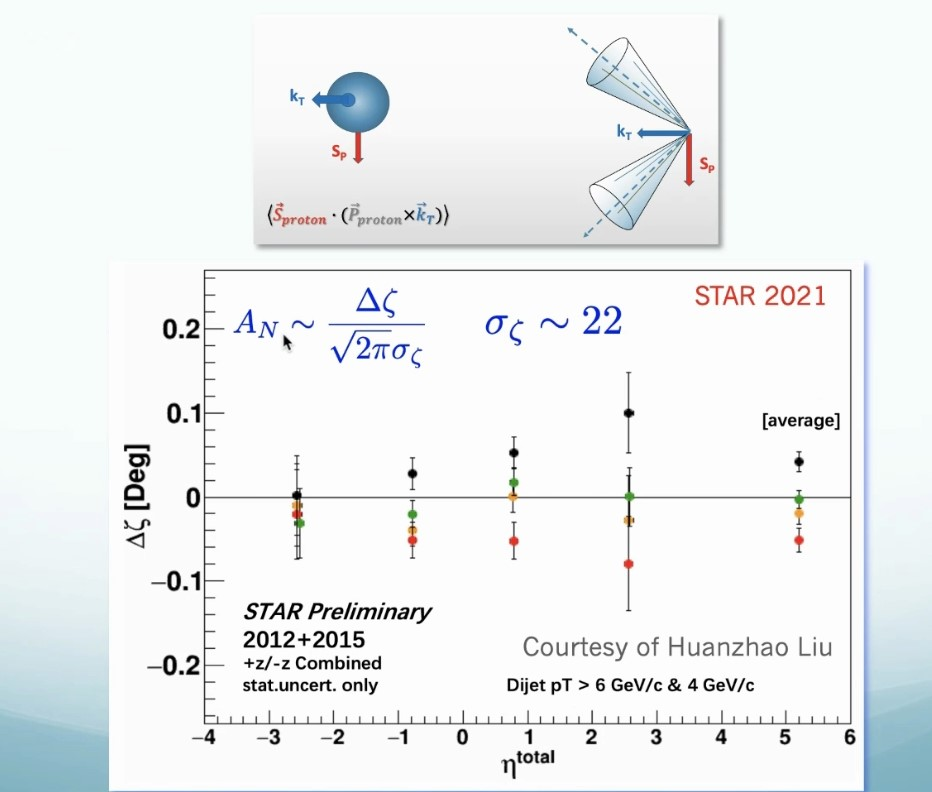
\includegraphics[scale=0.3]{dijet.jpg}
        \caption{dijet}
        \label{fig:side:b}
      \end{minipage}
 
\end{figure}
但这并不代表量子关系不存在,事实上我们可以先尝试看看测量强子的相互作用,我们分别采用两种方式:SIDIS和Drell-Yan
然后收集数据最终得到的结果可以看出其对称性,但是目前我们无论是进行single jet 或者是 dijet 都无法分辨出图中的u quark和d quark 产生的jet,
所以暂时只能将它们全部加起来,这也是我们看不出对称性的原因。
所以我们下面介绍Aharonov-Bohm effect来解决这个问题

\begin{figure}
    \begin{minipage}[t]{0.5\linewidth}
        \centering
        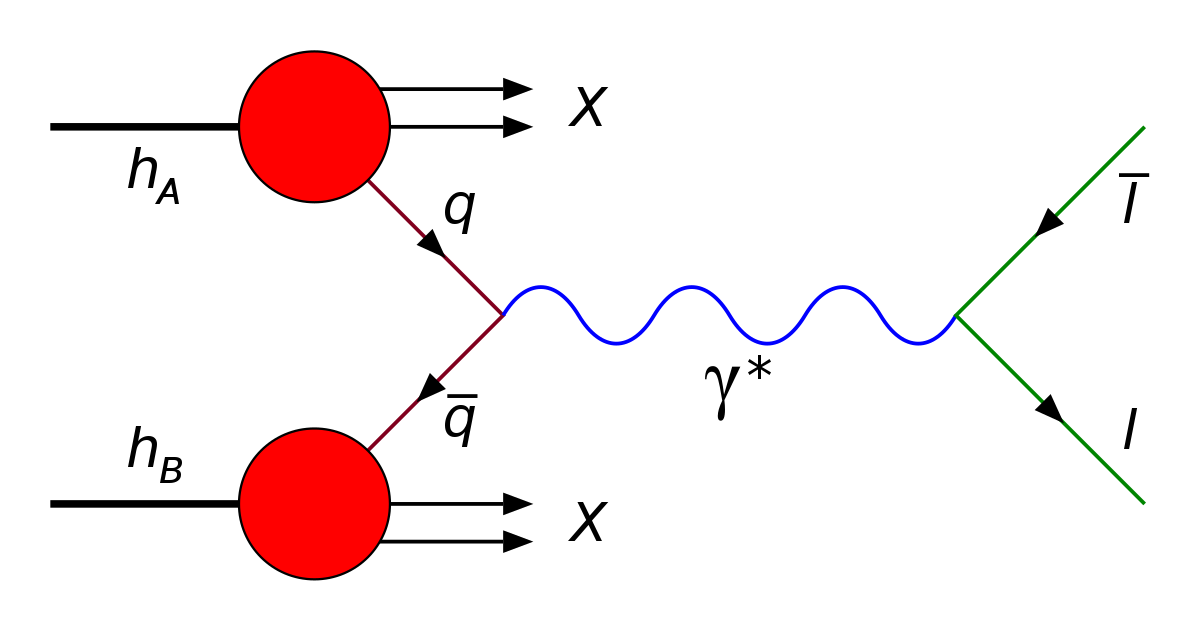
\includegraphics[scale=0.1]{drellyan.png}
        \caption{Drell-Yan}
        \label{fig:side:a}
      \end{minipage}%
      \begin{minipage}[t]{0.5\linewidth}
        \centering
        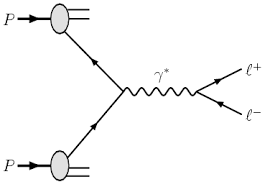
\includegraphics[scale=0.3]{SIDIS.png}
        \caption{SIDIS}
        \label{fig:side:b}
      \end{minipage}
\end{figure}
\begin{figure}
    \centering
    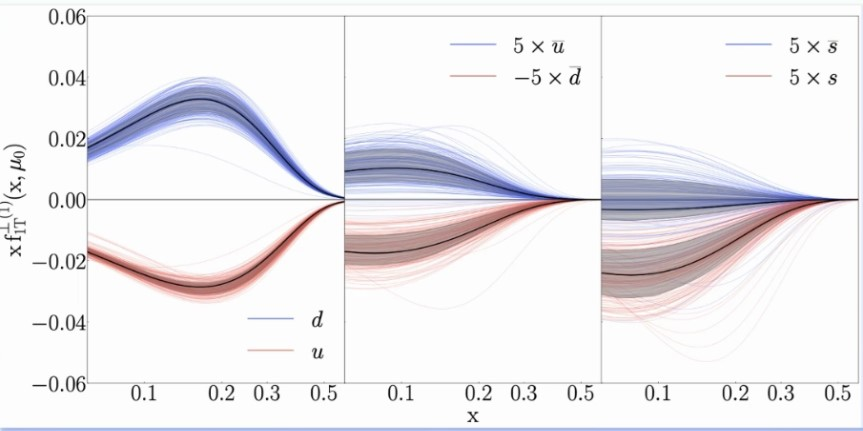
\includegraphics[width=8cm]{theta.jpg}
    \caption{asymmetry}    
\end{figure}


\subsection{Quantum phase:akin Aharonov-Bohm effect}
Aharonov-Bohm effect是一种量子力学现象,其中带电粒子受到电磁势 (φ, A) 的影响,尽管它们被限制在一个区域内磁场 B 和电场 E 为零。
其基本机制是电磁势与带电粒子波函数的复相耦合,干涉实验相应地说明了阿哈罗诺夫-玻姆效应。
Aharonov-Bohm effect的电磁效应的最初理论建议提出了一个实验,其中电荷沿着两条路径通过导电圆柱体,这在它们行进的区域中屏蔽了粒子免受外部电场的影响,
但仍然允许通过给圆柱体充电来施加与时间相关的电势。然而,事实证明这很难实现。取而代之的是,提出了一个不同的实验,
涉及一个被隧道势垒中断的环几何形状,一个恒定的偏置电压 V 与环的两半的电势相关。这种情况导致上述的 Aharonov-Bohm 相移,
并在 1998 年通过实验观察到

Aharonov-Bohm 效应在概念上很重要,因为它涉及将(麦克斯韦的)经典电磁理论重铸为规范理论的三个明显问题,
在量子力学出现之前,可以认为这是一种没有物理后果的数学重构。
这三个问题是:
势能是“物理的”还是仅仅是计算力场的便捷工具;
行动原则是否基本;
局部性原则。
Aharonov-Bohm effect证明即使在磁场为零的区域,仍旧会存在磁效应,然而,这并不能用来测量磁矢势,因为只有磁通量会出现在表达效应的公式里,
而且整个理论始终维持规范不变性。阿哈诺夫-波姆效应是量子力学和电动力学发展史上的重要实验,说明了量子力学的非局域性质。
运用到我们的jet,对于DIS quark 穿过reman的规范场从而产生phase rotation,$e^{i\phi}$$\phi = g_s \int_{path} \mathrm{d r}\cdot A$
,而且因为两者在光椎上的pass不一样,透过这样不同的phase,可以证明$Sivers function|_{DIS} = -Sivers function|_{DY}$
Sivers function大概是$f_{q / P^{\uparrow}}\left(x, \mathbf{k}_{\perp}, \vec{S}\right) \equiv f_{q / P}\left(x, k_{\perp}\right)-\frac{1}{M} f_{1 T}^{\perp q}\left(x, k_{\perp}\right) \vec{S} \cdot\left(\hat{p} \times \mathbf{k}_{\perp}\right)$

\begin{figure}
    \begin{minipage}[t]{0.5\linewidth}
        \centering
        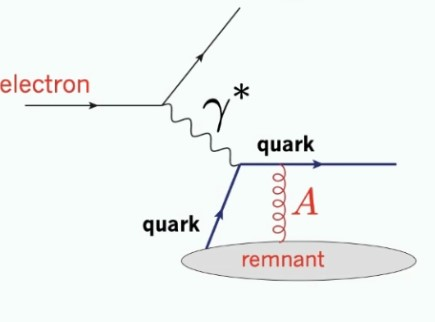
\includegraphics[scale=0.2]{DIS.jpg}
        \caption{DIS}
        \label{fig:side:a}
      \end{minipage}%
      \begin{minipage}[t]{0.5\linewidth}
        \centering
        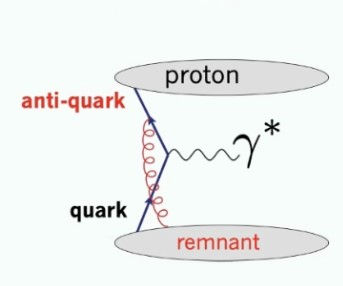
\includegraphics[scale=0.3]{drell.jpg}
        \caption{drell-yan}
        \label{fig:side:b}
      \end{minipage}
\end{figure}

而对于这些"Sivers"之间的关联可以影响我们对u quark和d quark的分类

\section{separate the quarks}

%idea:u and d have different charge, u quark have $+\frac{2}{3}e$, and the d quark have $-\frac{1}{3}e$
%if we can sum all the charge where in the end of the jet, we probabily can separate the u quark and d quark 
我们对于分离u quark 和 d quark 有一个猜想:因为u quark($+\frac{2}{3}e$) 和 d quark($-\frac{1}{3}e$) 有不同带电量
,所以如果我们可以把jet的末带电量全部加起来,我们就有可能分离u quark 和 d quark。
总带电量$Q_k \equiv \sum_{h\in jet}z^{\kappa}_hQ_h$, $z_h = \frac{p_{hT}}{p_{jT}},\kappa = 0.3,0.4,\dots,1.0$
\begin{figure}
    \centering
    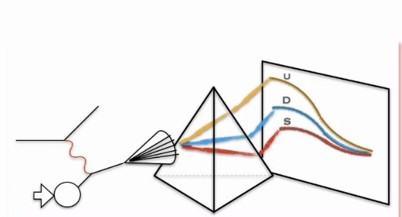
\includegraphics[width=8cm]{gamma.jpg}
    \caption{to get started,we decide to first look at jet production at the EIC}    
\end{figure}
\begin{figure}
    \centering
    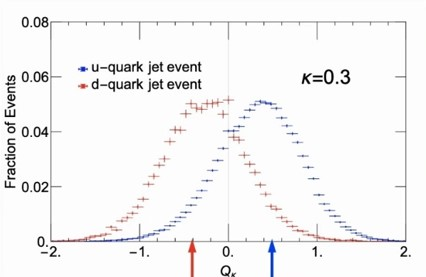
\includegraphics[width=8cm]{xi.jpg}
    \caption{jet charge distribution of u and d jets}    
\end{figure}
\begin{figure}
    \centering
    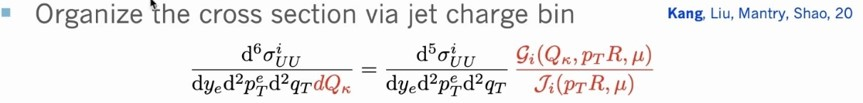
\includegraphics[width=8cm]{omega.jpg}
    \caption{organize the cross section via jet charge bin}    
\end{figure}
无发射电荷选项:去除了 d-夸克,变化很小,因此没有灵敏度
负发射电荷容器选项:更高的灵敏度
jet的例子表明。研究jet内部的成分可以给你新的见解jet子结构,
帮助我们实现其他方式无法实现的目标。
质子的 3D 成像:质子 → 夸克/胶子分布部分分布强子化:
夸克/胶子→强子碎裂函数
这个理论框架 • 称为极化射流。



在粒子物理里面,一般不在乎 jet的结构,因为只想寻找超出标准模型的粒子
关注QCD的原因是超出标准模型的粒子,产生的动量较小时,他们的衰减值就会很大,并且随着初态动量越来越大,他们的夹角会越来越小,
这样就会有一称为boosted partical的jet


\section{Conclusion}
本报告首先介绍了射流的产生原因以及会生成的物质(一般为胶子或夸克),射流是在 QCD 散射过程中产生的,产
生高横向动量夸克或胶子。微扰 QCD 计算可能在最终状态下具有有色部分,但只有最终产生的无色强子是通过实
验观察到的。
由於量子色動力學 (QCD) 限制只允許無色狀態,因此攜帶顏色電荷的粒子(例如夸克)不能以自由形式存在。當一個含有色荷的物體發生碎片時,
每個碎片都會帶走一些色荷。為了服從限制,這些碎片在它們周圍創造出其他有色物體,形成無色物體。這些物體的集合稱為射流,
因為碎片都傾向於沿同一方向行進,形成狹窄的粒子“射流”。射流在粒子探測器中被測量和研究,以確定原始夸克的性質。
其中也穿插了jet physics的应用例子,其中也介绍了许多学者们在不同方向的理论创新,包括质子成像,第六态有色玻璃凝聚物等等
接着简单介绍jet之后进入了规划实验部分,这里我们将两个质子相互作用他们的末态会产生一个射流,此时我们可以尝试对一个
质子探测我们需要的关联,对各个粒子进行观测建构出几个关系式,这一部分在理论范
围内使用了现象学的工作,这样我们就只需要和实验数据比对就行。
但其中发现此实验的不足之处会导致观测无法进行,对此,我们改进实验方法,在实验中进一步测量小的
横向动量,例如 dijet 中的横向动量的不平衡(见图b)从而建构一个有效的场理论。
我们接下来分别采用两种方式:SIDIS和Drell-Yan 然后收集数据。
但是目前我们无论是进行single jet 或者是 dijet 都无法分辨出图中的u quark和d
quark 产生的jet。也因此引入了Aharonov-Bohm effect并企图以此解决问题。
对于DIS quark 穿过reman的规范场从而产生phase rotation,$e^{i\phi}$$\phi = g_s \int_{path} \mathrm{d r}\cdot A$
,而且因为两者在光椎上的pass不一样,透过这样不同的phase,可以证明$Sivers function|_{DIS} = -Sivers function|_{DY}$
这样就可以分离前面提到的quarks了。
在粒子物理里面,一般不在乎 jet的结构,因为只想寻找超出标准模型的粒子
关注QCD的原因是超出标准模型的粒子,产生的动量较小时,他们的衰减值就会很大,并且随着初态动量越来越大,他们的夹角会越来越小,
这样就会有一称为boosted partical的jet

主要方法是利用quarks的带电量并透过总带电量$Q_k \equiv \sum_{h\in jet}z^{\kappa}_hQ_h$, $z_h = \frac{p_{hT}}{p_{jT}},\kappa = 0.3,0.4,\dots,1.0$
至此就可以完成前面的任务。



\end{spacing}

\bibliographystyle{IEEEtran}
\bibliography{jet-c-s}



\end{document}